\documentclass{standalone}
\usepackage{tikz}
\usetikzlibrary {arrows.meta}
\pagestyle{empty}

\begin{document}
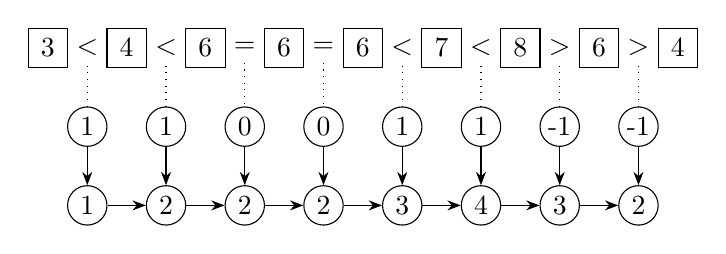
\begin{tikzpicture}

% Draw the array representation of the poplar heap 
\tikzstyle{every node}=[draw,shape=rectangle,minimum width=0.5cm,minimum height=0.5cm,anchor=center];
\foreach \x [count=\idx] in {3,4,6,6,6,7,8,6,4}
  \node (n\idx) at (\idx,5){\x};

\tikzstyle{every node}=[anchor=center];
\foreach \x [count=\idx] in {<,<,=,=,<,<,>,>}
  \node (s\idx) at (\idx+0.5,5){$\x$};

\tikzstyle{every node}=[draw,shape=circle,minimum size=0.5cm,inner sep=0pt,anchor=center];
\foreach \x [count=\idx] in {1,1,0,0,1,1,-1,-1}
  \node (r\idx) at (\idx+0.5,4){\x};

% Explicitly link the symbols to their order values
\foreach \x in {1,...,8}
   \draw[dotted] (s\x) -- (r\x);

\tikzstyle{every node}=[draw,shape=circle,minimum size=0.5cm,inner sep=0pt,anchor=center];
\foreach \x [count=\idx] in {1,2,2,2,3,4,3,2}
  \node (p\idx) at (\idx+0.5,3){\x};

% Link nodes to show the prefix sum
\foreach \x in {1,...,8}
   \draw[-Stealth] (r\x) -- (p\x);
\foreach[evaluate=\y using int(\x+1)] \x in {1,...,7}
  \draw[-Stealth] (p\x) -> (p\y);

% Draw the poplar heap nodes
% \node (n1) at (0,0) {3};
% \node (n2) at (1,0) {1};
% \node (n3) at (2,1) {6};
% \node (n4) at (3,0) {2};
% \node (n5) at (4,0) {4};
% \node (n6) at (5,1) {5};
% \node (n7) at (6,2) {7};

% Links between the nodes
% \draw (n7) -- (n6)
% (n7) -- (n3)
% (n6) -- (n5)
% (n6) -- (n4)
% (n3) -- (n2)
% (n3) -- (n1);


\end{tikzpicture}
\end{document}
